\documentclass[conference]{IEEEtran}

\usepackage{amsmath}
\usepackage{booktabs}
\usepackage{graphicx}
\usepackage{url}
\usepackage[hidelinks]{hyperref}

\title{Evaluating Logical Reasoning in Large Language Models Through Fine-Tuning and Neuro-Symbolic Bridging}

\author{\IEEEauthorblockN{Anonymous Author(s)}
\IEEEauthorblockA{Anonymous submission}}

\begin{document}
\maketitle

\begin{abstract}
Large language models can learn controlled deductive tasks, while neuro-symbolic pipelines seek to make their inferences executable and inspectable. Whether a symbolic bridge helps an already fine-tuned model depends on natural-language-to-logic translation fidelity. We present a matched evaluation on 200 held-out ProofWriter examples comparing a base Qwen3-1.7B model (C1), the same model with a checkpoint-250 LoRA adapter (C3), and that identical fine-tuned checkpoint routed through an NL2Logic-to-Z3 symbolic bridge whose verdict is the final answer (C4). Under strict scoring, with invalid outputs counted as errors, accuracy rises from 48.5\% in C1 to 82.5\% in C3, while macro-F1 rises from 0.251 to 0.826. Adding the bridge reduces accuracy to 49.5\% and macro-F1 to 0.459. C4 corrects 12 C3 errors but overturns 78 correct C3 predictions; the $-33.0$ percentage-point change is significant by exact McNemar testing ($p=5.20\times10^{-13}$). Although 89.5\% of bridge outputs execute, 80 executable verdicts are wrong and translation traces report widespread semantic divergence. In this implementation, translation fidelity is the principal bottleneck.
\end{abstract}

\begin{IEEEkeywords}
logical reasoning, large language models, fine-tuning, neuro-symbolic reasoning, semantic parsing, first-order logic, Z3
\end{IEEEkeywords}

\section{Introduction}
ProofWriter measures open-world deduction by pairing natural-language theories with conclusions labeled True, False, or Unknown \cite{tafjord2021proofwriter}. Neuro-symbolic systems such as Logic-LM and LINC translate language into formal representations before solver-based inference \cite{pan2023logiclm,olausson2023linc}; NL2Logic constrains this translation through a recursively constructed abstract syntax tree (AST) \cite{putra2026nl2logic}. Their success therefore depends on preserving the semantics of the original problem.

We isolate fine-tuning and bridge effects on one frozen 200-example ProofWriter subset \cite{tafjord2021proofwriter}. C1 is base direct inference, C3 is fine-tuned direct inference, and C4 routes the identical C3 checkpoint-250 adapter through the symbolic bridge, whose verdict becomes the final prediction. Accordingly, C1$\rightarrow$C3 measures fine-tuning, C3$\rightarrow$C4 measures the bridge, and C1$\rightarrow$C4 is descriptive only.

Our contributions are:
\begin{itemize}
    \item evidence that fine-tuning raises accuracy from 48.5\% to 82.5\%;
    \item a matched bridge comparison showing a fall to 49.5\%, with 12 corrections but 78 harmful overturns;
    \item trace-supported evidence that translation failures and semantically divergent executable logic explain the degradation; and
    \item a provenance-checked analysis that regenerates tables, intervals, and figures from canonical predictions.
\end{itemize}

\section{Related Work}
\subsection{Logical reasoning benchmarks}
ProofWriter operationalizes open-world deductive classification, records proof depth, and defines Unknown when neither a conclusion nor its contradiction is derivable \cite{tafjord2021proofwriter}. FOLIO provides naturally written arguments paired with first-order-logic annotations \cite{han2022folio}; it is not evaluated in this study.

\subsection{Language models and symbolic solvers}
Chain-of-thought prompting exposes intermediate natural-language reasoning steps \cite{wei2022cot}. Logic-LM translates problems into symbolic forms and can use solver feedback for refinement \cite{pan2023logiclm}; LINC delegates deduction to a theorem prover after semantic parsing \cite{olausson2023linc}. NL2Logic uses AST-guided recursive translation and deterministic two-pass compilation \cite{putra2026nl2logic}. We evaluate the latter translation pattern without comparing unmatched scores from prior systems.

\subsection{Efficient adaptation}
Qwen3 includes a 1.7B-parameter dense model \cite{qwen2025qwen3}. LoRA learns low-rank updates while pretrained weights remain frozen \cite{hu2021lora}; QLoRA combines such adapters with 4-bit NF4 quantization and paged optimization \cite{dettmers2023qlora}. We use these mechanisms to keep base-model identity fixed across conditions.

\section{System and Implemented Conditions}
\subsection{Task formulation}
ProofWriter uses open-world three-way classification \cite{tafjord2021proofwriter}. For a theory $T$ and hypothesis $h$, the target label is
\begin{equation}
y(T,h)=\begin{cases}
\text{True}, & T\models h,\\
\text{False}, & T\models \neg h,\\
\text{Unknown}, & \text{otherwise}.
\end{cases}
\end{equation}
All headline metrics use the three gold classes. A malformed or missing prediction is assigned to an Invalid prediction column and cannot match any gold label.

\subsection{C1: base direct}
C1 loads the pinned Qwen3-1.7B revision with NF4 quantization \cite{qwen2025qwen3,dettmers2023qlora} and deterministic decoding. An answer-only prompt requests True, False, or Unknown; no adapter or symbolic component is used.

\subsection{C3: fine-tuned direct}
C3 loads the same base revision and a ProofWriter LoRA adapter from checkpoint-250 \cite{tafjord2021proofwriter,hu2021lora}. Training uses NF4 quantization and paged optimization following the QLoRA design pattern \cite{dettmers2023qlora}. C3 uses the same direct prompt and evaluation path as C1.

\subsection{C4: fine-tuned neuro-symbolic bridge}
C4 loads the exact checkpoint-250 adapter used by C3. The canonical metadata identifies the descriptive prompt/schema configuration. Here, descriptive bridge means only this fixed natural-language schema variant; thereafter we use symbolic bridge. Following NL2Logic, it recursively constructs typed FOL AST nodes and compiles them in two passes \cite{putra2026nl2logic}, then queries the Z3 SMT solver \cite{demoura2008z3}. Entailment, contradiction, or neither maps to True, False, or Unknown, and that symbolic verdict is final.

\begin{figure*}[t]
\centering
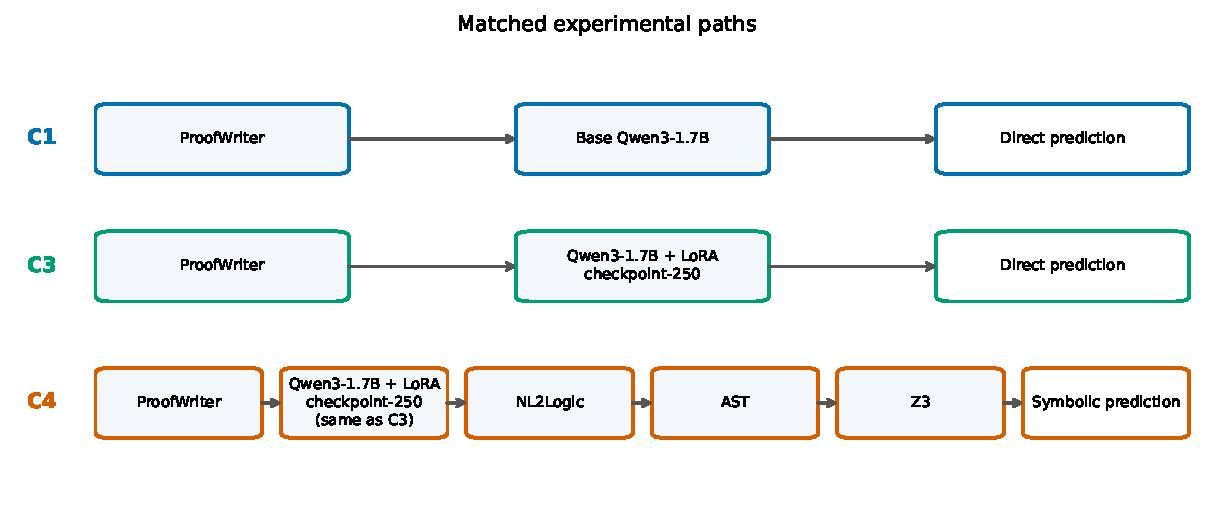
\includegraphics[width=0.96\textwidth]{figures/pipeline_overview.pdf}
\caption{Matched experimental paths. C3 and C4 use the same checkpoint-250 LoRA adapter \cite{hu2021lora}; only C4 adds the symbolic translation and solver path.}
\label{fig:pipeline}
\end{figure*}

\begin{table}[t]
\caption{Model and fine-tuning configuration.}
\label{tab:configuration}
\centering
\small
\begin{tabular}{ll}
\toprule
Item & Value \\
\midrule
Base model & Qwen3-1.7B \\
Quantization & NF4, FP16 compute \\
Training examples & 2,000 \\
Validation examples & 2,000 \\
LoRA rank / alpha / dropout & 16 / 32 / 0.05 \\
Learning rate / epochs & 2.0e-04 / 3 \\
Batch / accumulation & 1 / 16 \\
Optimizer / schedule & paged AdamW 8-bit / cosine \\
Selected adapter & checkpoint-250 \\
Bridge & descriptive NL2Logic $\rightarrow$ AST $\rightarrow$ Z3 \\
\bottomrule
\end{tabular}
\end{table}


\section{Experimental Setup}
\subsection{Data and canonical evidence}
The prepared ProofWriter source \cite{tafjord2021proofwriter} contains 585,552 training, 85,468 validation, and 174,476 test records. Controlled-language manifests select 2,000 training examples, 2,000 training-validation examples, and a 2,000-example held-out pool. The canonical evaluation is a label-and-QDep-stratified sample of 200 held-out examples using seed 42: 53 True, 53 False, and 94 Unknown.

The sole experimental source is the canonical ProofWriter run \cite{tafjord2021proofwriter} at \texttt{results/final200\_proofwriter}. Each condition contains 200 predictions with identical ordered identifiers, gold labels, and frozen subset hash. Provenance checks also require C3 and C4 to reference the same checkpoint-250 path; older and incomplete runs are excluded.

\begin{table}[t]
\caption{Dataset accounting. FOLIO is prepared but not evaluated.}
\label{tab:datasets}
\centering
\small
\begin{tabular}{lrrr}
\toprule
Dataset & Train & Validation & Held-out \\
\midrule
ProofWriter source & 585,552 & 85,468 & 174,476 \\
ProofWriter selected & 2,000 & 2,000 & 2,000 \\
ProofWriter canonical & -- & -- & 200 \\
FOLIO prepared & 896 & 105 & 203 \\
\bottomrule
\end{tabular}
\end{table}


\subsection{Metrics and statistical testing}
We report strict accuracy, macro precision/recall/F1, weighted F1, classwise scores, valid-output rate, and confusion matrices. Valid-only accuracy is reported only as a diagnostic and never replaces strict accuracy. For condition $c$ over $n=200$ examples,
\begin{equation}
\mathrm{Acc}_c=\frac{1}{n}\sum_{i=1}^{n}\mathbf{1}[\hat y_{c,i}=y_i].
\end{equation}
Confidence intervals use 10,000 paired bootstrap resamples with seed 42. The C3/C4 correctness difference is tested using the exact two-sided McNemar/binomial test on discordant pairs. The test concerns final correctness, not the internal cause of each error.

For intervention analysis we partition pairs into wrong$\rightarrow$correct (W$\rightarrow$C), correct$\rightarrow$correct, correct$\rightarrow$wrong (C$\rightarrow$W), and wrong$\rightarrow$wrong. The correction rate is W$\rightarrow$C divided by all C3 errors; the harm rate is C$\rightarrow$W divided by all C3 correct answers.

\section{Results}
\subsection{Fine-tuning effect: C1 to C3}
Table~\ref{tab:overall} and Fig.~\ref{fig:overall} show a large fine-tuning gain. Accuracy increases from 48.5\% (97/200) to 82.5\% (165/200), an absolute improvement of 34.0 percentage points. Macro-F1 increases from 0.251 to 0.826. The base model strongly defaults to Unknown: it achieves Unknown F1 of 0.646 but True F1 of 0.107 and False F1 of 0.000. Fine-tuning produces balanced classwise F1 scores of 0.854, 0.804, and 0.821 for True, False, and Unknown, respectively.

\begin{table*}[t]
\caption{Strict canonical ProofWriter results. Invalid outputs count as errors. Accuracy and validity are percentages.}
\label{tab:overall}
\centering
\small
\begin{tabular}{lrrrrr}
\toprule
Condition & Correct & Accuracy & Macro-F1 & Weighted F1 & Valid \\
\midrule
C1: base direct & 97/200 & 48.5 & 0.251 & 0.332 & 100.0 \\
C3: fine-tuned direct & 165/200 & \textbf{82.5} & \textbf{0.826} & 0.825 & 100.0 \\
C4: fine-tuned bridge & 99/200 & 49.5 & 0.459 & 0.491 & 89.5 \\
\bottomrule
\end{tabular}
\end{table*}


\begin{figure*}[t]
\centering
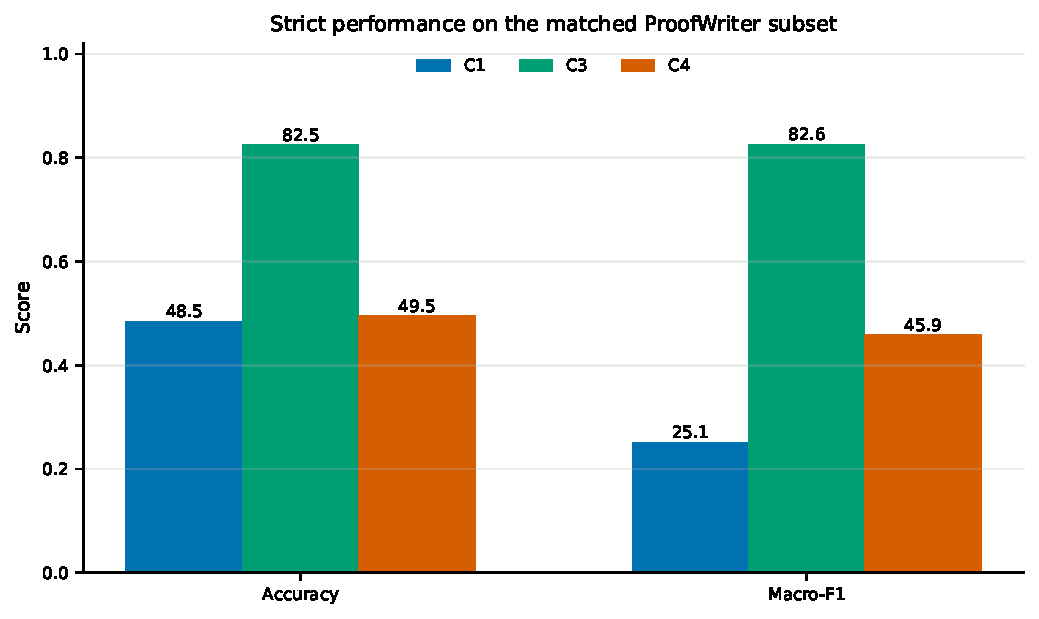
\includegraphics[width=0.78\textwidth]{figures/overall_comparison.pdf}
\caption{Strict accuracy and macro-F1. C1$\rightarrow$C3 isolates fine-tuning; C3$\rightarrow$C4 isolates the bridge.}
\label{fig:overall}
\end{figure*}

\begin{table}[t]
\caption{Per-class strict performance.}
\label{tab:perclass}
\centering
\scriptsize
\setlength{\tabcolsep}{3.2pt}
\begin{tabular}{llrrrr}
\toprule
Cond. & Class & Prec. & Rec. & F1 & Support \\
\midrule
C1 & True & 1.000 & 0.057 & 0.107 & 53 \\
C1 & False & 0.000 & 0.000 & 0.000 & 53 \\
C1 & Unknown & 0.477 & 1.000 & 0.646 & 94 \\
C3 & True & 0.880 & 0.830 & 0.854 & 53 \\
C3 & False & 0.837 & 0.774 & 0.804 & 53 \\
C3 & Unknown & 0.792 & 0.851 & 0.821 & 94 \\
C4 & True & 0.500 & 0.321 & 0.391 & 53 \\
C4 & False & 1.000 & 0.226 & 0.369 & 53 \\
C4 & Unknown & 0.526 & 0.745 & 0.617 & 94 \\
\bottomrule
\end{tabular}
\end{table}


\subsection{Bridge effect: C3 to C4}
Routing the same checkpoint through the bridge reduces strict accuracy from 82.5\% to 49.5\%, a 33.0-point decrease. Macro-F1 falls by 0.367, from 0.826 to 0.459. The paired bootstrap 95\% confidence interval for the accuracy difference is $[-0.410,-0.245]$, and exact McNemar testing on 90 discordant pairs gives $p=5.20\times10^{-13}$. The direct model makes 35 errors; C4 makes 101, corresponding to a 188.6\% increase in the error rate. C1 and C4 differ by only one accuracy point, but that contrast is descriptive because both adaptation and inference path differ.

C4 produces a valid label for 179 examples (89.5\%). Conditional accuracy on those valid outputs is 55.3\%, still far below C3. Thus, invalid outputs explain 21 errors but not the majority of the 66 additional errors.

\begin{table}[t]
\caption{Bootstrap intervals (10,000 paired resamples).}
\label{tab:statistics}
\centering
\scriptsize
\begin{tabular}{lrr}
\toprule
Quantity & Estimate & 95\% CI \\
\midrule
C1 accuracy & 0.485 & [0.415, 0.555] \\
C1 macro-F1 & 0.251 & [0.208, 0.299] \\
C3 accuracy & 0.825 & [0.770, 0.875] \\
C3 macro-F1 & 0.826 & [0.769, 0.876] \\
C4 accuracy & 0.495 & [0.430, 0.565] \\
C4 macro-F1 & 0.459 & [0.380, 0.534] \\
C4$-$C3 accuracy & -0.330 & [-0.410, -0.245] \\
\midrule
McNemar discordant & 90 & $p=5.20e-13$ \\
\bottomrule
\end{tabular}
\end{table}


\subsection{Confusion structure and reasoning depth}
Figure~\ref{fig:confusions} shows that C3 resolves True and False with few cross-class mistakes, while C4 shifts many cases toward Unknown: 29 of 53 True and 34 of 53 False instances become Unknown. C4 also maps 14 Unknown examples to True and yields 21 invalid predictions. This pattern is consistent with information being lost or distorted before symbolic inference.

\begin{figure*}[t]
\centering
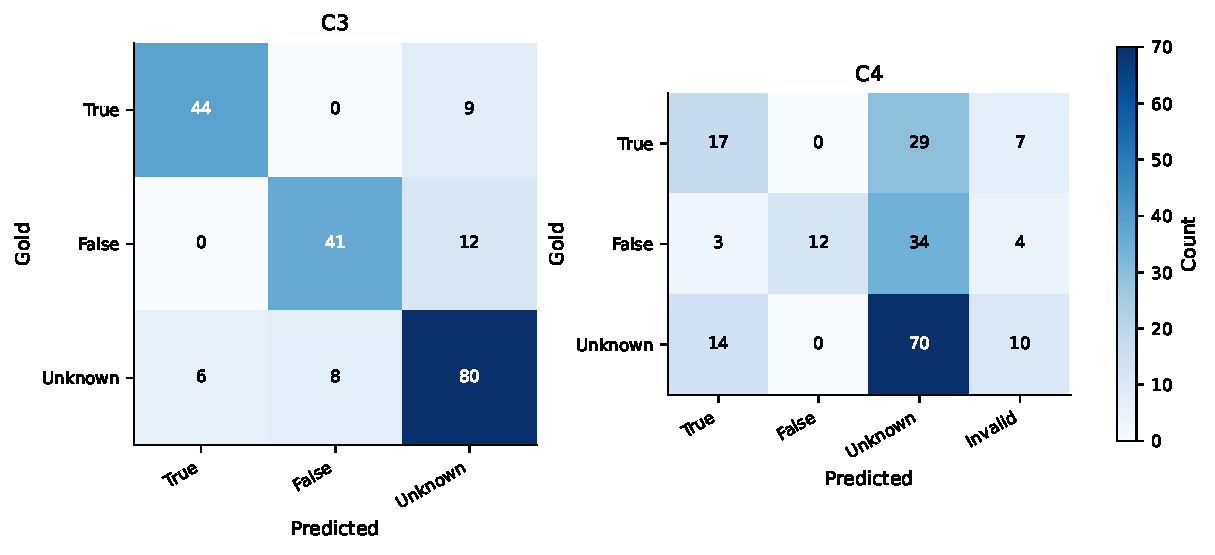
\includegraphics[width=0.90\textwidth]{figures/confusion_matrices.pdf}
\caption{Strict confusion matrices for C3 and C4. Invalid is a prediction outcome, not a fourth gold class.}
\label{fig:confusions}
\end{figure*}

QDep metadata support an observational depth analysis. C3 leads at every grouped depth: it moves from 96.2\% at depth 0 to 26.7\% at depth 3 and 75.0\% in the four-example 4+ group. C4 moves from 69.2\% at depth 0 to 6.7\% at depth 3 and 0\% at 4+. The imbalanced and very small tail groups preclude causal conclusions.

\section{Intervention and Error Analysis}
\subsection{Corrections versus harmful overturns}
The paired transition counts in Table~\ref{tab:interventions} reveal why aggregate performance collapses. C4 corrects 12 of C3's 35 errors, a 34.3\% correction rate. However, it overturns 78 of C3's 165 correct answers, a 47.3\% harm rate. Eighty-seven examples remain correct and 23 remain wrong, yielding 66 net lost corrections. A useful bridge policy would need to identify when translation and symbolic execution are trustworthy; no such policy exists in this implementation.

\begin{table}[t]
\caption{Paired C3$\rightarrow$C4 intervention outcomes.}
\label{tab:interventions}
\centering
\small
\begin{tabular}{lr}
\toprule
Outcome & Count \\
\midrule
Wrong $\rightarrow$ correct & 12 \\
Correct $\rightarrow$ correct & 87 \\
Correct $\rightarrow$ wrong & 78 \\
Wrong $\rightarrow$ wrong & 23 \\
\midrule
Correction rate & 34.3\% \\
Harm rate & 47.3\% \\
Net corrections & -66 \\
\bottomrule
\end{tabular}
\end{table}


\subsection{Bridge reliability and failure modes}
Twenty C4 examples fail before solver execution: 11 are malformed and nine are schema invalid. Of the remaining 180, 179 execute successfully in Z3 and one produces inconsistent premises. Nevertheless, 80 of the 179 executable cases (44.7\%) end with an incorrect symbolic verdict.

Translation diagnostics provide direct evidence of mismatch. The recorded semantic-equivalence field is \texttt{different} for 158 examples and unavailable for 42; exact and normalized logic matches are zero. Parser recovery fields appear in 1,122 trace steps spanning 193 examples. These are step-level recovery events, not 1,122 failed examples, but their prevalence shows that permissive fallback behavior is central to the translation path. We do not attribute every executable error to a particular parser step: solver-correct reasoning over semantically altered logic, hypothesis mistranslation, rule mistranslation, and predicate-argument inconsistency can produce the same final symptom.

\begin{table}[t]
\caption{C4 bridge reliability and outcomes ($n=200$).}
\label{tab:bridge}
\centering
\small
\begin{tabular}{lrr}
\toprule
Stage/outcome & Count & Rate (\%) \\
\midrule
Schema/parser/AST valid & 180 & 90.0 \\
Compilation success & 180 & 90.0 \\
Z3 executable & 179 & 89.5 \\
Correct symbolic verdict & 99 & 49.5 \\
Executable but incorrect & 80 & 40.0 \\
Malformed/schema invalid & 20 & 10.0 \\
Inconsistent premises & 1 & 0.5 \\
\bottomrule
\end{tabular}
\end{table}


\subsection{Latency}
Direct inference is inexpensive: mean end-to-end latency is 0.136 seconds for C1 and 0.228 seconds for C3. C4 averages 22.60 seconds (median 21.27, 95th percentile 38.71), about 99 times C3 latency. Across the 200 examples, C4 consumes roughly 75.3 minutes and records 11,726 recursive parser call requests and 3,960 model invocations. The current bridge therefore trades both accuracy and latency for symbolic executability.

\section{Discussion}
The C1/C3 comparison shows that the 2,000-example LoRA adaptation is the dominant positive factor in this experiment: it replaces C1's strong Unknown bias with balanced True, False, and Unknown performance. The matched C3/C4 comparison then localizes the degradation to the added translation-and-solver path, not to a different checkpoint.

The bridge is not uniformly harmful---it fixes 12 errors---but its 78 harmful overturns show that the current translator cannot reliably identify when its formalization preserves the source theory. Future work should test semantic consistency, predicate and variable binding, and calibrated abstention as new matched conditions. This conclusion is specific to the implemented bridge and does not imply that neuro-symbolic methods generally harm reasoning.

\section{Limitations and Threats to Validity}
The canonical subset contains 200 examples from one controlled benchmark and one random seed. Although matched design supports paired inference, confidence intervals remain wide for small depth groups. ProofWriter's synthetic language limits generalization to naturally occurring text. The base model, adapter, prompts, and bridge are single implementations; results do not establish that fine-tuning always dominates neuro-symbolic reasoning or that NL2Logic generally fails.

The trace fields can establish well-formedness, execution, fallback activity, and recorded semantic mismatch, but they cannot uniquely assign causal responsibility for every incorrect verdict. Moreover, C4 has no retain/correct/abstain policy, so this study evaluates complete routing through the bridge rather than selective verification.

An additional natural-language benchmark is prepared for future work, but no matched prediction-level evaluation exists; no performance is reported. No matched self-check or symbolic-only baseline is available.

\section{Conclusion}
On a matched 200-example ProofWriter evaluation, LoRA fine-tuning raises Qwen3-1.7B accuracy from 48.5\% to 82.5\%. Routing that same checkpoint through the implemented symbolic bridge reduces accuracy to 49.5\%. The bridge corrects 12 direct errors but breaks 78 correct answers; parser failures explain 20 invalid cases, while many executable verdicts remain wrong. The bounded conclusion is that translation fidelity, not symbolic reasoning in general, is the bottleneck in this implementation.

\section*{Reproducibility Statement}
All reported values are regenerated from the raw JSONL files in the frozen canonical directory. The analysis validates row count, identifier order, gold-label identity, subset hash, and checkpoint identity before computing results. It writes one canonical results object consumed by CSV audits, LaTeX tables, and figures. Bootstrap sampling uses seed 42 and 10,000 replicates. No model inference is rerun to build this paper.

\bibliographystyle{IEEEtran}
\bibliography{references}

\end{document}
